\documentclass[10pt]{article}
\usepackage[english]{babel}
\usepackage{../../../meta-inf/lib/naproche}
\usepackage{amssymb}
\usepackage{mathtools} % for \coloneq

\usepackage{stex-highlighting}
\providebool{emph} % "\newbool{emph}" does not work...
\setbool{emph}{false}
\colorlet{emphcolor}{violet}
\let\oldemph\emph
\renewcommand\emph[1]{\setbool{emph}{true}\ifbool{forthel}{\textcolor{emphcolor}{\itshape#1}}{\oldemph{#1}}\setbool{emph}{false}}
\renewcommand{\varemph}[1]{\ifbool{emph}{\textcolor{emphcolor}{#1}}{\textcolor{black}{#1}}}

\usepackage[right=6cm,left=3cm,bottom=3cm,marginparwidth=5cm]{geometry}

\usepackage{fancyhdr}
\renewcommand{\sectionmark}[1]{\markboth{#1}{}} 
\def\libarchive{}
\pagestyle{fancy}
\fancyhead[L]{\libarchive}
\fancyhead[C]{\nouppercase\leftmark}  % section title
\fancyhead[R]{\thepage}               % page number
\fancyfoot[C]{}                       % No page number in footer

\usepackage[nobottomtitles]{titlesec}
\titlespacing*{\section}{0pt}{30pt}{0pt}
\titlespacing*{\subsection}{0pt}{30pt}{0pt}
\titlespacing*{\subsubsection}{0pt}{30pt}{0pt}

\documentclass[12pt,oneside]{book}

\usepackage[foundations]{../../lib/tex/naproche}
\usepackage{../../lib/tex/libraries}
\usepackage{graphicx}
\usepackage{float}
\usepackage{caption}
\usepackage{footnote}

\makesavenoteenv{tabular} % Make footnotes work in tabular environments


\title{Foundations of Mathematics}
\author{Marcel Schütz}
\date{2022}

\begin{document}
  \maketitle

  \tableofcontents

  \begin{figure}[H]
    \centering
    \fbox{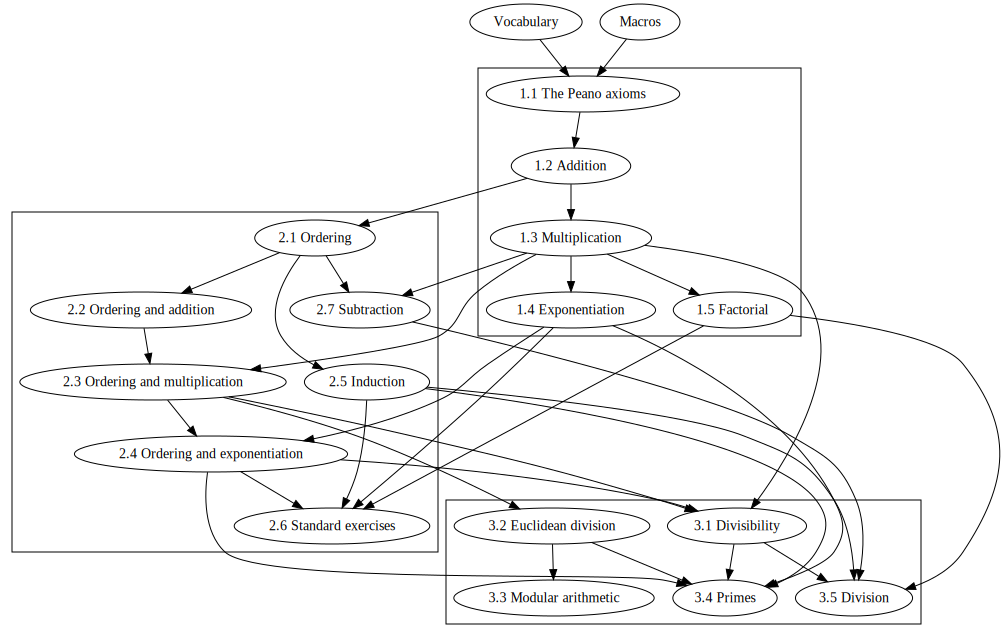
\includegraphics[width=0.9\linewidth]{./dependency-graph/graph.png}}
    \caption*{Interdependencies of the chapters}
  \end{figure}


  \section*{Introduction}

  This is a library providing a foundation of mathematics based on a
  Kelley-Morse like class theory with urelements.
  It introduces common operations on classes like unions or intersections
  (\cref{chapter:classes}) together with detailed proofs of their algebraic
  properties (\cref{chapter:computation-laws-for-classes}), the symmetric
  difference of two classes (\cref{chapter:symmetric-difference}) and the
  notions of ordered pairs and Cartesian products
  (\cref{chapter:pairs-and-products}) as well as proofs of the algebraic
  properties of the latter (\cref{chapter:computation-laws-for-products}).
  Moreover, it provides common operations on maps (\cref{chapter:maps}), various
  properties of images and preimages (\cref{chapter:image-and-preimage}) and the
  notions of injectivity, surjectivity, bijectivity
  (\cref{chapter:injections-surjections-bijections}) and invertibility of maps
  (\cref{chapter:invertible-maps}).
  The library provides an axiom system characterizing sets (\cref{chapter:sets})
  and, furthermore, it covers the notions of binary relations
  (\cref{chapter:binary-relations}), fixed-points of subset preserving maps
  (\cref{chapter:fixed-points}), including and equinumerosity
  (\cref{chapter:equinumerosity}).

  As two famous results it includes the Knaster-Tarski fixed point theorem
  (\cref{FOUNDATIONS_12_8420450166112256}) and the Cantor-Schröder-Bernstein
  theorem (\cref{FOUNDATIONS_13_1913663275401216}).

  \paragraph*{Usage.}
  At the very beginning of each chapter you can find the name of its source
  file, e.g. \path{foundations/sections/01_classes.ftl.tex} for
  \cref{chapter:classes}. This filename can be used to import the chapter via
  \Naproche's \texttt{readtex} instruction to another ForTheL text, e.g.:
  \begin{center}
    \verb`[readtex \path{foundations/sections/01_classes.ftl.tex}]`
  \end{center}

  \paragraph*{Checking times.}
  The checking times for each of the chapters may vary from computer to
  computer, but on mid-range hardware they are likely to be similar to those
  given in table below:

  \begin{center}
    \begin{tabular}{c|c|c}

      & \multicolumn{2}{c}{\textbf{Checking time}}
      \\
      \textbf{Chapter}
      & \textbf{without dependencies}     & \textbf{with dependencies}
      \\ \hline
      \ref{chapter:classes}
      & 00:04 min                         & 00:04 min
      \\
      \ref{chapter:computation-laws-for-classes}
      & 00:12 min                         & 00:16 min
      \\
      \ref{chapter:symmetric-difference}
      & 00:32 min                         & 00:48 min
      \\
      \ref{chapter:pairs-and-products}
      & 00:08 min                         & 00:12 min
      \\
      \ref{chapter:computation-laws-for-products}
      & 01:36 min                         & 01:56 min
      \\
      \ref{chapter:maps}
      & 01:13 min                         & 01:25 min
      \\
      \ref{chapter:image-and-preimage}
      & 01:28 min                         & 02:53 min
      \\
      \ref{chapter:injections-surjections-bijections}
      & 00:38 min                         & 02:03 min
      \\
      \ref{chapter:invertible-maps}
      & 02:20 min                         & 04:23 min
      \\
      \ref{chapter:sets}
      & 02:17 min                         & 06:40 min
      \\
      \ref{chapter:binary-relations}
      & 00:14 min                         & 06:54 min
      \\
      \ref{chapter:fixed-points}
      & 00:33 min                         & 07:13 min
      \\
      \ref{chapter:equinumerosity}
      & 01:48 min                         & 09:01 min
    \end{tabular}
  \end{center}


  \subfile{sections/01_classes.ftl.tex}
  \subfile{sections/02_computation-laws-for-classes.ftl.tex}
  \subfile{sections/03_symmetric-difference.ftl.tex}
  \subfile{sections/04_pairs-and-products.ftl.tex}
  \subfile{sections/05_computation-laws-for-products.ftl.tex}
  \subfile{sections/06_maps.ftl.tex}
  \subfile{sections/07_image-and-preimage.ftl.tex}
  \subfile{sections/08_injections-surjections-bijections.ftl.tex}
  \subfile{sections/09_invertible-maps.ftl.tex}
  \subfile{sections/10_sets.ftl.tex}
  \subfile{sections/11_binary-relations.ftl.tex}
  \subfile{sections/12_fixed-points.ftl.tex}
  \subfile{sections/13_equinumerosity.ftl.tex}
\end{document}

\usepackage{amssymb}

\newcommand{\Nat}{\mathbb{N}}
\newcommand{\Prime}{\mathbb{P}}
\renewcommand{\succ}{\textrm{succ}}
\newcommand{\pred}{\textrm{pred}}
\newcommand{\add}{\textrm{add}}
\newcommand{\mul}{\textrm{mul}}
\renewcommand{\exp}{\textrm{exp}}
\newcommand{\fac}{\textrm{fac}}
\renewcommand{\div}{\mathop{\textrm{div}}}
\renewcommand{\mod}{\mathop{\textrm{mod}}}

\begin{document}
  \begin{imports}
    \begin{forthel}
      %[prove off][check off]
      [read \path{libraries/source/arithmetics/divisibility.ftl.tex}]
      [read \path{libraries/source/arithmetics/modular-arithmetics.ftl.tex}]
      %[prove on][check on]
    \end{forthel}
  \end{imports}


  \section*{Prime Numbers}

  \begin{forthel}
    \begin{definition}[id=ARITHMETIC_10_5450464558579712,printid]
      Let $n$ be a natural number.
      $n$ is prime iff $n > 1$ and $n$ has no nontrivial divisors.
    \end{definition}

    Let $n$ is compound stand for $n$ is not prime.
    Let a prime number stand for a natural number that is prime.
  \end{forthel}

  \begin{forthel}
    \begin{definition}[id=ARITHMETIC_10_3834705971511296,printid]
      $\Prime$ is the class of all prime numbers.
    \end{definition}
  \end{forthel}

  \begin{forthel}
    \begin{proposition}[id=ARITHMETIC_10_7801379464675328,printid]
      Let $n$ be a natural number such that $n > 1$.
      Then $n$ is prime iff every divisor of $n$ is a trivial divisor of $n$.
    \end{proposition}
  \end{forthel}

  \begin{forthel}
    \begin{proposition}[id=ARITHMETIC_10_3606185106210816,printid]
      Let $n$ be a natural number such that $n > 1$.
      Then $n$ has a prime divisor.
    \end{proposition}
    \begin{proof}
      Define $\Phi = \{ n' \in \Nat \mid$ if $n' > 1$ then $n'$ has a prime divisor $\}$.

      Let us show that for every $n' \in \Nat$ if $\Phi$ contains all
      predecessors of $n'$ then $\Phi$ contains $n'$.
        Let $n' \in \Nat$.
        Assume that $\Phi$ contains all predecessors of $n'$.
        We have $n' = 0$ or $n' = 1$ or $n'$ is prime or $n'$ is composite.

        Case $n' = 0$ or $n' = 1$. Trivial.

        Case $n'$ is prime. Obvious.

        Case $n'$ is composite.
          Take a nontrivial divisor $m$ of $n'$.
          Then $1 < m < n'$.
          $m$ is contained in $\Phi$.
          Hence we can take a prime divisor $p$ of $m$.
          Then we have $p \mid m \mid n'$.
          Thus $p \mid n'$.
          Therefore $p$ is a prime divisor of $n'$.
        End.
      End.

      Thus every natural number belongs to $\Phi$ (by \printref{ARITHMETIC_04_3609801697263616}).
    \end{proof}
  \end{forthel}

  \begin{forthel}
    \begin{definition}[id=ARITHMETIC_10_463197419077632,printid]
      Let $n, m$ be natural numbers.
      $n$ and $m$ are coprime iff for all nonzero natural numbers $k$ such that $k \mid n$ and $k \mid m$ we have $k = 1$.
    \end{definition}

    Let $n$ and $m$ are relatively prime stand for $n$ and $m$ are coprime.
    Let $n$ and $m$ are mutually prime stand for $n$ and $m$ are coprime.
    Let $n$ is prime to $m$ stand for $n$ and $m$ are coprime.
  \end{forthel}

  \begin{forthel}
    \begin{proposition}[id=ARITHMETIC_10_5776394594287616,printid]
      Let $n, m$ be natural numbers.
      $n$ and $m$ are coprime iff $n$ and $m$ have no common prime divisor.
    \end{proposition}
    \begin{proof}
      Case $n$ and $m$ are coprime.
        Let $p$ be a prime number such that $p \mid n$ and $p \mid m$.
        Then $p$ is nonzero and $p \neq 1$.
        Contradiction.
      End.

      Case $n$ and $m$ have no common prime divisor.
        Assume that $n$ and $m$ are not coprime.
        Let $k$ be a nonzero natural number such that $k \mid n$ and $k \mid m$.
        Assume that $k \neq 1$.
        Consider a prime divisor $p$ of $k$.
        Then $p \mid k \mid n,m$.
        Hence $p \mid n$ and $p \mid m$.
        Contradiction.
      End.
    \end{proof}
  \end{forthel}

  \begin{forthel}
    \begin{proposition}[id=ARITHMETIC_10_7212152851005440,printid]
      Let $n, m$ be natural numbers and $p$ be a prime number.
      If $p$ does not divide $n$ then $p$ and $n$ are coprime.
    \end{proposition}
    \begin{proof}
      Assume $p \nmid n$.
      Suppose that $p$ and $n$ are not coprime.
      Take a nonzero natural number $k$ such that $k \mid p$ and $k \mid n$.
      Then $k = p$.
      Hence $p \mid n$.
      Contradiction.
    \end{proof}
  \end{forthel}

  \begin{forthel}
    \begin{proposition}[id=ARITHMETIC_10_8313676557713408,printid]
      Let $n, m$ be natural numbers and $p$ be a prime number.
      If $p \mid n \cdot m$ then $p \mid n$ or $p \mid m$.
    \end{proposition}
    \begin{proof}
      Assume $p \mid n \cdot m$.

      Case $p \mid n$. Trivial.

      Case $p \nmid n$.
        Define $\Phi = \{ k \in \Nat \mid k \neq 0$ and $p \mid k \cdot m \}$.
        Then $p \in \Phi$ and $n \in \Phi$.
        Hence $\Phi$ contains some natural number.
        Thus we can take $a \in \Phi$ such that $a \leq k$ for all $k \in \Phi$.

        Let us show that $a$ divides all elements of $\Phi$.
          Let $k \in \Phi$.
          Take natural numbers $q, r$ such that $k = (a \cdot q) + r$ and $r < a$ (by \printref{ARITHMETIC_08_7743986617810944}).
          Indeed $a$ is nonzero.
          Then $k \cdot m
            = ((q \cdot a) + r) \cdot m
            = ((q \cdot a) \cdot m) + (r \cdot m)$.
          We have $p \mid k \cdot m$.
          Hence $p \mid ((q \cdot a) \cdot m) + (r \cdot m)$.

          We can show that $p \mid r \cdot m$.
            We have $p \mid a \cdot m$.
            Hence $p \mid (q \cdot a) \cdot m$.
            Indeed $((q \cdot a) \cdot m) = q \cdot (a \cdot m)$. %!
            Take $A = (q \cdot a) \cdot m$ and $B = r \cdot m$. %!
            Then $p \mid A + B$ and $p \mid A$.
            Thus $p \mid B$ (by \printref{ARITHMETIC_07_1076947887063040}).
            Indeed $p, A$ and $B$ are natural numbers.
            Consequently $p \mid r \cdot m$.
          End.

          Therefore $r = 0$.
          Indeed if $r \neq 0$ then $r$ is an element of $\Phi$ that is less than $a$.
          Hence $k = q \cdot a$.
          Thus $a$ divides $k$.
        End.

        Then we have $a \mid p$ and $a \mid n$.
        Hence $a = p$ or $a = 1$.
        Thus $a = 1$.
        Indeed if $a = p$ then $p \mid n$.
        Then $1 \in \Phi$.
        Therefore $p \mid 1 \cdot m = m$.
      End.
    \end{proof}
  \end{forthel}
\end{document}
